
\documentclass[12pt]{amsart}
\usepackage{geometry} % see geometry.pdf on how to lay out the page. There's lots.
\geometry{a4paper} % or letter or a5paper or ... etc
% \geometry{landscape} % rotated page geometry
\usepackage{graphicx} %插入图片的宏包
\usepackage{float} %设置图片浮动位置的宏包
\usepackage{subfigure} %插入多图时用子图显示的宏包

% See the ``Article customise'' template for come common customisations

\title{}
\author{}
\date{} % delete this line to display the current date

%%% BEGIN DOCUMENT
\begin{document}

\section{Original Design}

\begin{figure}[H] %H为当前位置,!htb为忽略美学标准,htbp为浮动图形
\centering %图片居中
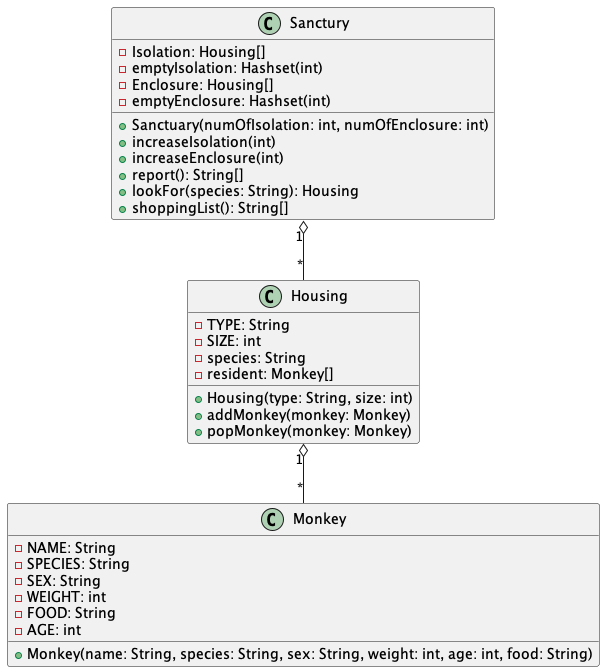
\includegraphics[width=1\textwidth]{uml.png} %插入图片,[]中设置图片大小,{}中是图片文件名
\end{figure}

\newpage

\section{Monkey}

\begin{table}[htbp]
   %\topcaption{Table captions are better up top} % requires the topcapt package
   \begin{tabular}{@{} lcr @{}} % Column formatting, @{} suppresses leading/trailing space

      Testing construction      & Input & Expected \\
         Constructor with invalid name       & Monkey(``'', ``drill'', ``Male'', 80, 12, ``eggs'')     &  IllegalArgumentException \\
         Constructor with invalid species       & Monkey(``good'', ``ok'', ``Male'', 80, 12, ``eggs'')     &  IllegalArgumentException \\
         Constructor with invalid sex       & Monkey(``good'', ``drill'', ``ok'', 80, 12, ``eggs'')     &  IllegalArgumentException \\
         Constructor with invalid weight       & Monkey(``good'', ``drill'', ``Male'', -80, 12, ``eggs'')     &  IllegalArgumentException \\
         Constructor with invalid age       & Monkey(``good'', ``drill'', ``Male'', 80, -12, ``eggs'')     &  IllegalArgumentException \\
         Constructor with invalid food       & Monkey(``good'', ``drill'', ``Male'', 80, 12, ``apples'')     &  IllegalArgumentException \\
         Constructor with valid input       & Monkey(``good'', ``drill'', ``Male'', 80, 12, ``eggs'')     &  None \\
    \end{tabular}
\end{table}

%\newpage

\section{Housing}
% Requires the booktabs if the memoir class is not being used

\begin{table}[htbp]
   %\topcaption{Table captions are better up top} % requires the topcapt package
   \begin{tabular}{@{} lcr @{}} % Column formatting, @{} suppresses leading/trailing space

      Testing construction      & Input & Expected \\
         Constructor with invalid type       & Housing(``ok'', 10)     &  IllegalArgumentException \\
         Constructor with invalid size       & Housing(``Isolation'', -1)     &  IllegalArgumentException \\
         Constructor with valid type and size       & Housing(``Isolation'', 10)     &  None \\
         Constructor with valid type and size       & Housing(``Enclosure'', 10)     &  None \\
          & & \\
       Testing addMonkey() & Input & Expected \\
       Add a monkey & addMonkey(monkeyA) & None\\
          & & \\
       Testing popMonkey() & Input & Expected \\
       Pop a monkey & popMonkey(monkeyA) & None\\
    \end{tabular}
\end{table}

\section{Sanctuary}

\begin{table}[htbp]
   %\topcaption{Table captions are better up top} % requires the topcapt package
   \begin{tabular}{@{} lcr @{}} % Column formatting, @{} suppresses leading/trailing space

      Testing construction      & Input & Expected \\
         Constructor with invalid input       & Sanctuary(-1, 1)     &  IllegalArgumentException \\
         Constructor with invalid input       & Sanctuary(1, -1)     &  IllegalArgumentException \\
         Constructor with valid input       & Sanctuary(1, 1)     &  None \\
          & & \\
       Testing increaseIsolation() & Input & Expected \\
       increase one each time & increaseIsolation() & None\\
          & & \\
       Testing increaseEnclosure() & Input & Expected \\
       increase one each time & increaseEnclosure() & None\\
          & & \\
       Testing report() & Input & Expected \\
       report species housed & report() & String[] in alphabetical order\\
          & & \\
       Testing lookFor() & Input & Expected \\
       look up for a special species & lookFor(``species name'') & a Housing object\\
          & & \\
       Testing shoppingList() & Input & Expected \\
       print a list for favorite food & shoppingList() & String[]\\
    \end{tabular}
\end{table}

\newpage

\section{Final Design}
\begin{figure}[htbp] %H为当前位置,!htb为忽略美学标准,htbp为浮动图形
\centering %图片居中
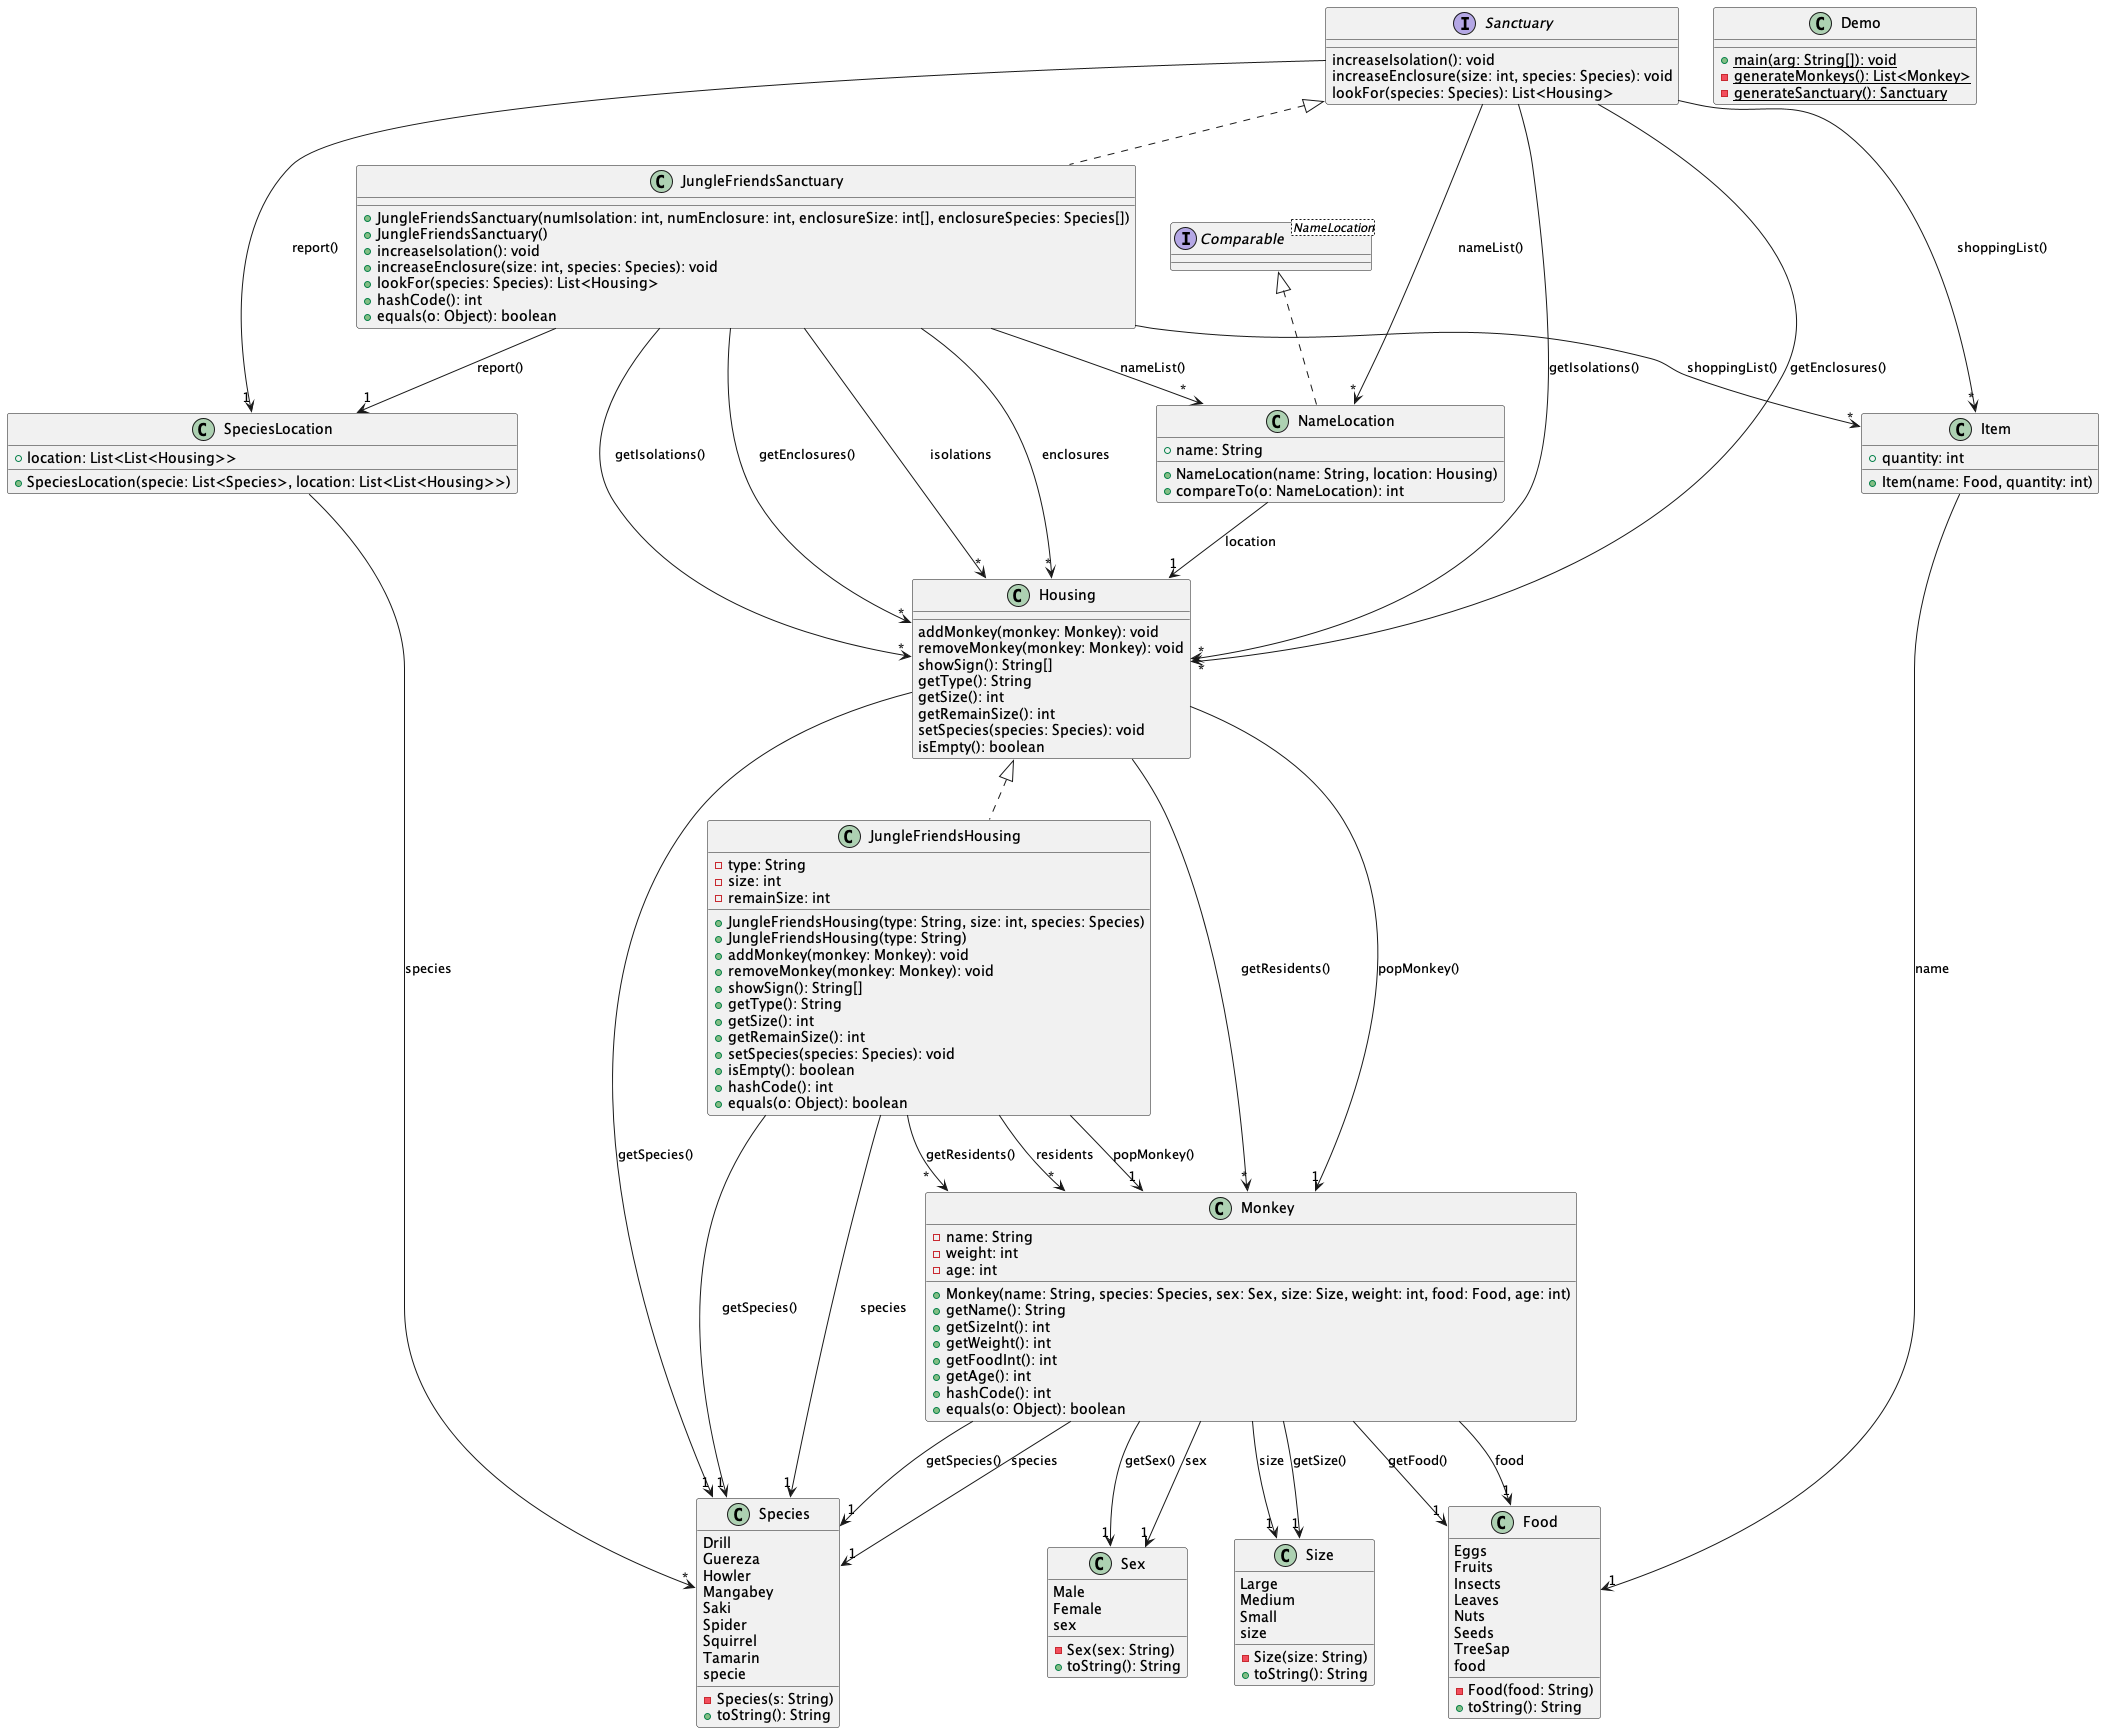
\includegraphics[width=1\textwidth]{sanctuary.png} %插入图片,[]中设置图片大小,{}中是图片文件名
\end{figure}

\newpage
\section{Monkey}

\begin{table}[htbp]
   %\topcaption{Table captions are better up top} % requires the topcapt package
   \begin{tabular}{@{} lcr @{}} % Column formatting, @{} suppresses leading/trailing space

      Testing construction      & Input & Expected \\
         Constructor with invalid name       & Monkey("", Species.Drill, Sex.Female, Size.Large,
      10, Food.Eggs, 10)    &  IllegalArgumentException \\
         Constructor with invalid species       & Monkey("name", Species.Drill, Sex.Female, Size.Large,
      0, Food.Eggs, 10);     &  IllegalArgumentException \\
         Constructor with invalid sex       & Monkey("name", Species.Drill, Sex.Female, Size.Large,
      10, Food.Eggs, -1);     &  IllegalArgumentException \\
    \end{tabular}
\end{table}

%\newpage
\newpage
\section{Housing}
% Requires the booktabs if the memoir class is not being used

\begin{table}[htbp]
   %\topcaption{Table captions are better up top} % requires the topcapt package
   \begin{tabular}{@{} lcr @{}} % Column formatting, @{} suppresses leading/trailing space

      Method Tested      & Input & Expected \\
         Constructor with invalid type       & JungleFriendsHousing("any", 1, Species.Drill);    &  IllegalArgumentException \\
         Constructor with incompatible type and species       & JungleFriendsHousing("Isolation", 1, Species.Drill);     &  IllegalArgumentException \\
         Constructor with incompatible type       & JungleFriendsHousing("Enclosure");     &  IllegalArgumentException \\
         Constructor with incompatible type and species       & JungleFriendsHousing("Enclosure", -1, Species.Drill);     &  IllegalArgumentException \\
          & & \\
       testAddMonkey & tmp.addMonkey(this.monkey); & IllegalArgumentException\\
          & & \\
       testRemoveMonkey & this.iso.removeMonkey(this.monkey); & IllegalArgumentException \\
       testPopMonkey & if the poped is equal to the entered & None\\
       testPopMonkey & It's empty after pop & None\\
       & &\\
       testShowSign & Test on empty house & IllegalArgumentException\\
       testShowSign & Test on nonempty house & String of name, sex and food\\
    \end{tabular}
\end{table}

\newpage
\section{Sanctuary}

\begin{table}[htbp]
   %\topcaption{Table captions are better up top} % requires the topcapt package
   \begin{tabular}{@{} lcr @{}} % Column formatting, @{} suppresses leading/trailing space

      Method Tested      & Input & Expected \\
         Constructor with invalid input       & Negative number of isolation     &  IllegalArgumentException \\
         Constructor with invalid input       & Negative number of enclosure     &  IllegalArgumentException \\
         Constructor with invalid input       & Incompatible enclosure size species length    &  IllegalArgumentException \\
          & & \\
       testIncreaseIsolation & tmp.increaseIsolation();& None\\
          & & \\
       testIncreaseEnclosure & tmp.increaseEnclosure(5, Species.Drill); & None\\
       testIncreaseEnclosure & tmp.increaseEnclosure(-1, Species.Drill); & IllegalArgumentException\\
          & & \\
       testReport & SpeciesLocation report = tmp.report(); & A SpeciesLocation Object\\
          & & \\
     testLookFor &tmp.lookFor(this.monkey.getSpecies()).get(0) & List of Housing\\
          & & \\
       testShoppingList& List<Item> shopList = tmp.shoppingList(); & List of Item objects \\
    \end{tabular}
\end{table}



\end{document}